\documentclass[]{article}
\usepackage{tikz}
\usepackage{amsmath}

\title{Dimensional Analysis of Perturbation Height in Incompressible Stokes Flow}
\author{Nat Lund}

\begin{document}
\maketitle

Observe:
\vspace{1em}

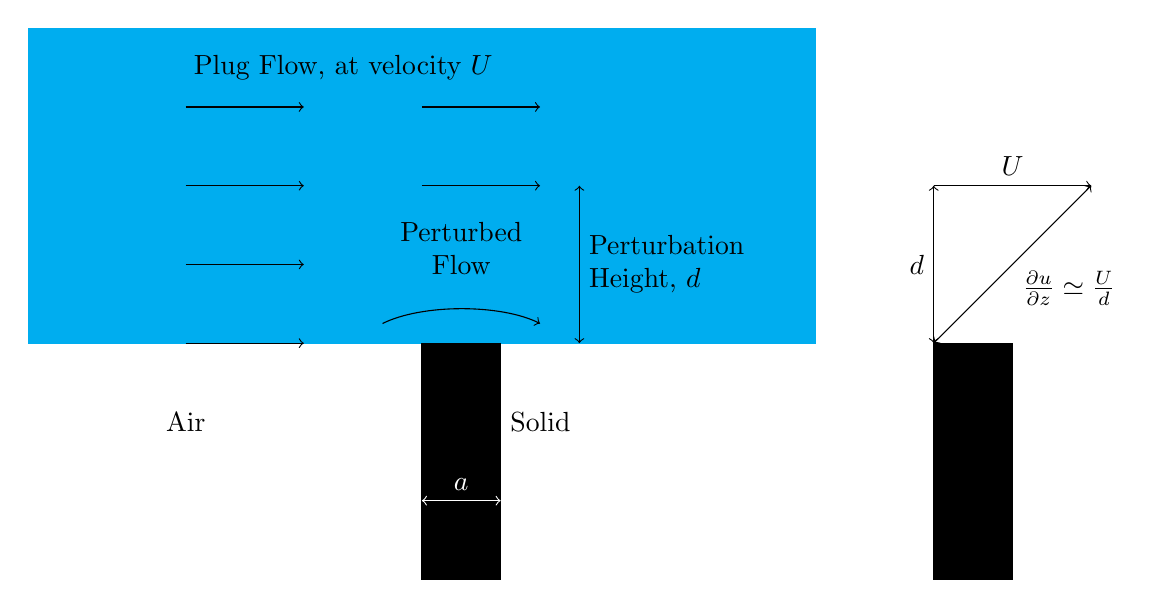
\begin{tikzpicture}

\filldraw[color=cyan] (-5,4) rectangle (5,0);
\filldraw (0,0) rectangle (1,-3);
\node at (-3,-1) {Air};
\node at (1,-1) [right] {Solid};

\draw [color=white, <->] (0,-2) -- node[above] {$a$} (1,-2);

\node at (-1,3.5) {Plug Flow, at velocity $U$};

\foreach \z in {0,1,2,3}
   \draw [->] (-3, \z) -- (-1.5, \z);
   
\node at (0.5,1.2) [align=center] {Perturbed\\Flow};
\draw [->] (-0.5,0.25) .. controls (0,0.5) and (1,0.5) .. (1.5, 0.25);
\foreach \z in {2,3}
   \draw [->] (0, \z) -- (1.5, \z);

\draw [<->] (2,0) -- node[right,align=left]{Perturbation\\Height, $d$} (2,2);


\filldraw (6.5,0) rectangle +(1,-3);
\draw [<->](6.5,0) -- node[left] {$d$} +(0,2);
\draw [->](6.5,2) -- node[above] {$U$} +(2,0);
\draw [<->](6.5,0) --  +(2,2);
\node at (7.5,0.7) [right] {$\frac{\partial u}{\partial z} \simeq \frac{U}{d}$};

\end{tikzpicture}
\vspace{1em}

What is perturbation height $d$?

It will be a function of some fundamental physical parameters:
\begin{itemize}
    \item Ridge width $a$
    \item Velocity $U$
    \item Viscosity $\eta$
    \item Density $\rho$
    \item Pressure $p$
\end{itemize}

In other words $d = g(a, U, \eta, \rho, p )$. $\;\;$ Or equivalently, $f(d,a,U,\eta, \rho, p)=0$.

Dimensionally,
\[d = [m],\;\; a = [m],\;\; U = [ms^{-1}],\;\; \eta = [kg s^{-1} m^{-1}],\;\; \rho = [kg m^{-3}], \;\;\; p = [kg m^{-1} s^{-2}] \]

\[ d = [m],\;\;\; a = [m],\;\;\; U = \left[\frac{m}{s} \right],\;\;\;
 \eta = \left[\frac{kg}{ms} \right],\;\;\; \rho = \left[\frac{kg}{m^{3}} \right]
 ,\;\;\; p = \left[ \frac{kg}{m s^{2}} \right] \]
 
We also know that the fluid is incompressible, creeping flow.  As such, it obeys the continuity equation:
\[ \frac{\partial u}{\partial x} + \frac{\partial v}{\partial z} = 0 \]
And Stokes equations:
\[ \mu \nabla^2 u = \frac{\partial p}{\partial x} \;\;\; \text{and} \;\;\;
\mu \nabla^2 v = \frac{\partial p}{\partial z} \]

These equations put a constraint on the relationships between the physical variables...

\end{document}